\section{Review of research methodology}
\begin{figure}[htbp]
    \centering
    % \columnwidth forces it to perfectly fit the width of one single column
    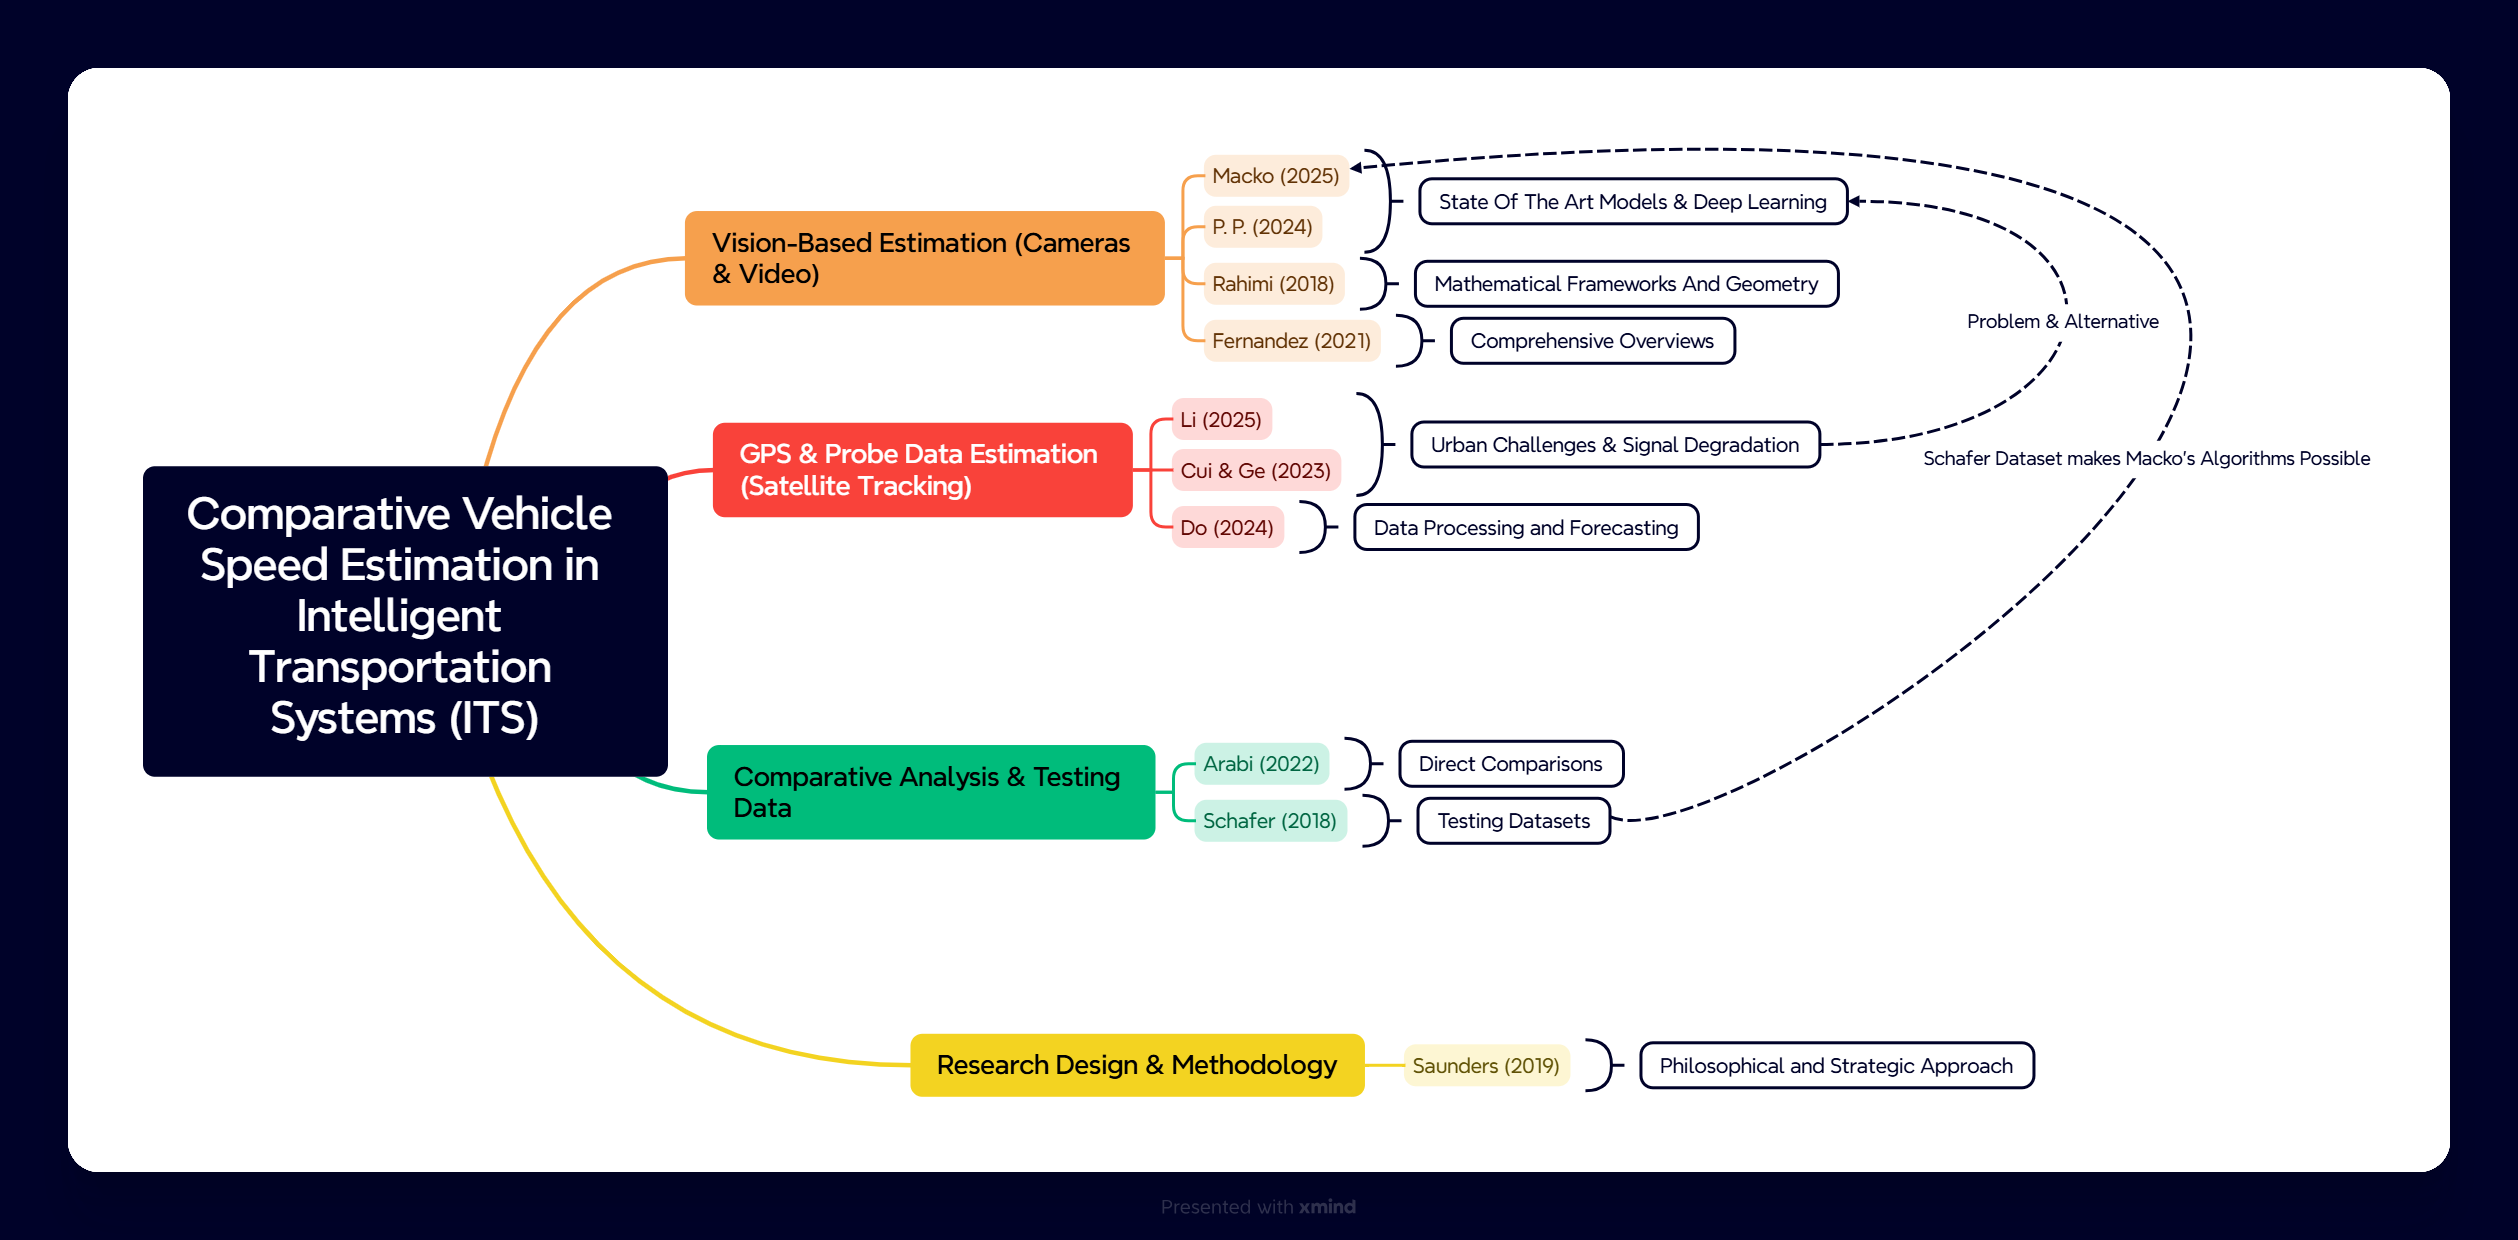
\includegraphics[width=\columnwidth]{includes/literaturemap.png}
    \caption{Literature Map}
    \label{fig:LiteratureMap}
\end{figure}
In the field of Intelligent Transportation Systems (ITS), the selected methodology fundamentally determines the accuracy of speed estimation. Looking into this research area, you can spot two main methods. Researchers focusing on vision-based speed estimation usually take an experimental, deductive approach based on positivism. Their methods generally entails the collection of primary data through edge-computing cameras, utilising geometric transformations (such as Inverse Perspective Mapping) or pixel-tracking algorithms to ascertain speed based on observable physical displacement.

Conversely, researchers looking at GPS probe data often go for a second, more numbers-driven way of analysing things. Their methodology utilises extensive datasets comprising historical, crowdsourced vehicle trajectories. Instead of conducting real-time physical experiments, their focus is predominantly on statistical modelling, noise mitigation, and using map-matching algorithms to fix those multi-path errors that pop up in city areas.

\subsection{Testing Strategies in the Chosen Context}
To implement these methods, a review of the literature identifies three principal testing strategies utilised by researchers to evaluate speed estimation frameworks.

The initial approach is what they call Controlled Closed-Circuit Testing, whereby researchers typically initiate testing within controlled, sterilised environments. They drive their specially equipped vehicles at set speeds around a closed track. This method effectively removes extraneous variables such as traffic occlusion or unpredictable civilian driving behaviour, thereby facilitating a concentrated focus on the mathematical principles underpinning the vision or GPS algorithms.

The second approach is known as `In-The-Wild' Highway Deployment. To check how well it scales, researchers put cameras on busy motorway overpasses. This testing method relies on obtaining a substantial sample size of uninstrumented civilian vehicles. The speed info from the vision system is then compared with big-picture GPS data from third-party companies to see how accurate it is in real-world conditions and how much delay there might be.

The third method involves Synthetic Simulation (Digital Twins). Researchers are progressively utilising advanced rendering engines to artificially produce accurate bounding boxes and tracking data in fake extreme weather scenarios that would be hard to mimic in real life. This methodology serves as an effective means of advancing the mathematical boundaries of speed estimation algorithms.

\subsection{Experimental Variables and Hypothesis Validation}
No matter what testing approach you use, researchers need to carefully control and tweak certain experimental variables to prove their ideas. When it comes to independent variables in vision-based studies, they often mess around with the camera angle (pitch and yaw), how far away the camera is from the target, and things like lighting and weather to see how solid the system is. Conversely, in studies involving GPS technology, the primary independent variable manipulated is the `polling rate', defined as the frequency at which the GPS receiver records a coordinate.

Accompanying these inputs, the universally measured dependent variable across all studies is the calculated velocity, expressed in kilometres per hour (km/h) or metres per second (m/s), along with the error margin, which they usually measure using Root Mean Square Error (RMSE) or Mean Absolute Percentage Error (MAPE).

Furthermore, to institute control variables and prove an alternative hypothesis, such as the proposal that a vision-based model shows greater accuracy than conventional GPS. This is usually done by arming test vehicles with super-calibrated Real-Time Kinematic (RTK) GPS or using LiDAR speed guns. Finally, by isolating these variables, researchers can definitively discover the specific parameters under which their speed estimation models remain valid.

\subsection{Distinguishing Between Academic and Non-Academic Material}
When we're looking at these variables and methods, it's important to clearly distinguish between well-tested academic research driven by the industry that isn't academically reviewed. Academic material sourced from peer-reviewed journals, these studies offer transparent methods, publicly accessible datasets (such as BrnoCompSpeed), and standard error metrics. They candidly acknowledge limitations, including camera calibration drift and GPS multipath errors.

Non-academic material, such as industry white papers and promotional reports from ITS hardware manufacturers, offer valuable insights into real-world adoption. However, they often lack methodological transparency. Frequently, they present ``best-case scenario'' accuracy figures without sufficiently detailing the experimental constraints, thereby rendering them unsuitable for establishing a scientific baseline.

\subsection{Recommended Peer-Reviewed Articles}
The following five peer-reviewed articles establish the methodological foundation for the comparison of vision and GPS techniques, each representing distinct layers of Saunders' Research Onion. 

\cite{macko2025efficient} operate firmly within a positivist paradigm, employing an experimental strategy through the employment of YOLO object detection in conjunction with vanishing point geometry. This study exemplifies contemporary standards for quantitative methodologies and procedures, avoiding reliance solely on fixed road-width assumptions.

Additionally \cite{arabi2022comparison} offer a highly pertinent comparative methodology in their work ``Comparison of the GPS and Camera Distance Estimation''. Their research demonstrates a deductive approach, establishing a rigorous framework for experimental validation by utilising RTK GPS as an infallible ground truth to test alternative hypotheses against monocular camera estimations.

Furthermore, \cite{fernandez2021vision} is integral to its archival research strategy, delineating the methodological evolution in data collection and analysis techniques, from fundamental background subtraction to sophisticated deep learning and optical flow methods.

To effectively contextualise the alternative approach in \cite{do2024enhanced}, this study focuses extensively on the specific techniques and procedures necessary for overseeing the inherent noise and low polling rates characteristic of continuous GPS trajectory data, relying heavily on large-scale cross-sectional data collection.

Lastly, \cite{rahimi2018vehicle} employs a strict monomethod quantitative approach, explicitly detailing the mathematical methodology involving virtual intrusion lines and frame-by-frame displacement. This represents a practical realisation of the innermost layers of the research onion, offering a methodology directly applicable to the development of bounding box prototype designs.

\subsection{Critical Literature Arguments and Knowledge Gaps}
A critical synthesis of the literature reveals distinct trade-offs between the two methodologies. Vision-based approaches are often praised for their strong localisation and perfect coverage, capturing every passing vehicle. However, the literature frequently disparages these systems for their fragility. Mathematical calibration is readily compromised by camera vibrations, and accuracy diminishes substantially during nighttime or adverse weather conditions.

Conversely, GPS probe data methods are esteemed for their continuous, network-wide coverage and resilience to visual environmental factors. Nonetheless, GPS studies frequently emphasise notable spatial inaccuracies within urban canyon environments, primarily due to signal multipath errors, and these methods are often characterised by low rates.

\subsubsection{Identifying The Knowledge Gap}
While there's plenty of research looking at vision systems in really controlled settings and GPS on open roads, there's still a big gap when it comes to comparing their performance all at once in busy, complicated city environments. Most studies investigate a single technology while presuming the other to be an infallible ground truth. There is a conspicuous absence of empirical research that rigorously evaluates a hybrid tracking methodology, such as integrating YOLO bounding boxes for primary detection with precise pixel displacement techniques, measured directly against consumer-grade GPS data within a real-world urban bottleneck scenario.